\textbf{ID:} UC09 (Review for Approval) \\
\textbf{Scope:} CS Automated Information Timeline \\
\textbf{Level:} User Goal \\
\textbf{Stakeholders and Interests:}
\begin{itemize}
    \item Faculty: A person that works for the university and is interested in gaining visibility of their post and/or event.
    \item Administrator/Reviewer: A person that works for the university and is interested in reviewing and approving requests for system content additions.
\end{itemize}
\textbf{Preconditions:}
\begin{itemize}
    \item Administrator/Reviewer a has been identified and authenticated.
    \item Notification n has been created and persisted.
    \item n.event, n.post, or n.media has been set.
\end{itemize}
\textbf{Postconditions:}
\begin{itemize}
    \item Notification n.entity was identified as either a Post, Event, or Media.
    \item n.entity.status was set to either “Approved” or “Rejected”.
    \item If the review was favorable, n.entity.status was set to “Approved”.
    \item If the review was unfavorable, n.entity.status was set to “Rejected”.
    \item n.reviewer was set to a.
    \item n.entity was persisted.
\end{itemize}
\textbf{Main Success Scenario:}
\begin{enumerate}
    \item Administrator/Reviewer, a, gets all notifications.
    \item For each Notification, n, in notifications, Administrator/Reviewer, a, performs manual review of the Post, Event, or Media attached to Notification, n.
    \item Administrator/Reviewer, a, updates the Post, Event, or Media that was attached to Notification, n, to either “Approved” or “Rejected”.
    \item If the review is favorable, n.event.status, n.post.status, or n.media.status is set to “Approved”.
    \item If the review is not favorable, n.event.status, n.post.status, or n.media.status is set to “Rejected”.
    \item The system persists the updated Post, Event, or Media with the status set by Administrator/Reviewer, a.
    \item The system associates Administrator/Reviewer, a, with Notification n.
    \item Notification, n, is persisted.
    \item The Event, Post, or Media is persisted.
\end{enumerate}
\textbf{Extensions:} \\
2a. There are multiple objects, Post, Event, or Media, attached to Notification n.
\begin{itemize}
    \item Administrator/Reviewer, a, deletes Notification, n.
\end{itemize}
\textbf{Special Requirements:} None \\
\textbf{Technology and Data Variation List:}
\begin{itemize}
    \item Notification n.post is set and of Post type; n.event and n.media are null.
    \item Notification n.event is set and of Event type; n.post and n.media are null.
    \item Notification n.media is set and of Media type; n.post and n.event are null.
\end{itemize}
\textbf{Frequency of Occurrence:} Could be nearly continuous. \\

\begin{figure}[H]
    \centering
    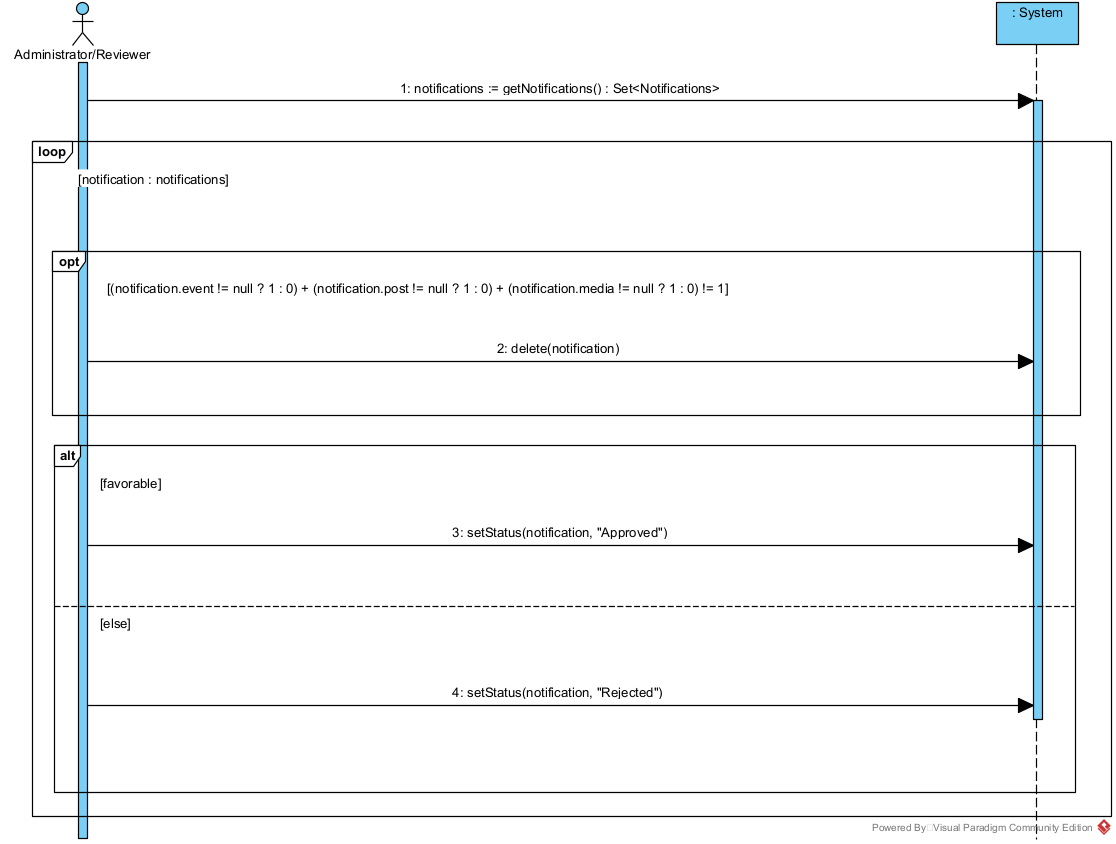
\includegraphics[width=0.8\textwidth]{images/SSD-UC09-ReviewForApproval.png}
    \centering
    \caption{System Sequence Diagram: Review For Approval}
\end{figure}

\textbf{Operation:} getNotifications() \\
\textbf{Cross References:} UC09 (Review for Approval) \\
\textbf{Preconditions:}
\begin{itemize}
    \item Admin/Reviewer, a, has been identified and authenticated.
    \item Notification, n, has been created and persisted.
    \item Notification n.entity has been set to Post p, Event e, and/or Media m.
\end{itemize}
\textbf{Postconditions:} None \\

\textbf{Operation:} deleteNotification(notification: Notification) \\
\textbf{Cross References:} UC09 (Review for Approval) \\
\textbf{Preconditions:}
\begin{itemize}
    \item Admin/Reviewer, a, has been identified and authenticated.
    \item Notification, n, has been created and persisted.
    \item Notification n.entity has been set to Post p, Event e, and/or Media m.
\end{itemize}
\textbf{Postconditions:}
\begin{itemize}
    \item Association n.entity was disassociated.
    \item All entities, Post p, Event e, and/or Media m, from association n.entity were removed from persistence and destroyed.
    \item Notification, n, was removed from persistence and destroyed.
\end{itemize}

\textbf{Operation:} setStatus(status: String) \\
\textbf{Cross References:} UC09 (Review for Approval) \\
\textbf{Preconditions:}
\begin{itemize}
    \item Admin/Reviewer, a, has been identified and authenticated.
    \item Notification, n, has been created and persisted.
    \item n.reviewer has been set to Admin/Reviewer a.
    \item n.entity has been set to one of Post p, Event e, or Media m.
\end{itemize}
\textbf{Postconditions:}
\begin{itemize}
    \item Notification n.entity.status was set to status.
    \item Notification n.reviewer was set to a.
    \item Notification, n, was persisted.
\end{itemize}
